\chapter{Introduction}\label{chap:intro}\index{Introduction}


\medskip

In this dissertation we will investigate Credit Derivative Pricing Surfaces. We will
review the pricing mechanisms for these products and survey the current state of the art.   
In Chapter~\ref{chap:review} we review the credit derivatives market, introduce various credit derivatives products.  We attempt to refer to the 2007 Credit Crisis where appropriate as this is of direct consequence to the Credit Derivative marketplace. 

Who seeks to use Credit Derivatives and transfer credit risk? \cite{Gib2007} details the type of counterparty within credit derivative deals with the largest category of buyers being reporting dealers. \cite{Gib2007} also discusses the three market participants for credit derivatives, namely, commercial banks, investment banks, and investors.  Commercial banks seek to manage their risk exposure. For this they might use a single name CDS to diffuse credit risk of an issuer with whom they have significant exposure.   
An Investment bank would use credit derivatives to manage the credit risk of underwriting securities before it sells them to market, for example in the warehousing of a number of mortgage loans in the run up to securitisation. From 2004 CDSs on asset backed securities grew to \$125 billion in 2007 and these allowed underwriters to buy credit protection on these warehoused MBS deals. Finally, investors will purchase credit derivatives with many different strategies ranging from buy-and-hold (pension funds) to active trading (hedge funds), though even these distinctions can be vague.  

The International Swaps and Derivatives Association (ISDA) 2007 year-end survey of the over-the-counter derivatives market stated that credit default swaps (CDS), including single-name CDS, baskets and portfolios of credit and index trades, was the fastest growing asset class. The notional amount outstanding of CDSs increased 81 percent over the previous year to \$62.2 trillion from \$34.5 trillion at year-end 2006.\footnote{Source: http://www.securitiesindustry.com/news/22270-1.html}


\section{Credit Derivative Products}

The Credit Default Swap (CDS) is the most widely traded Credit Derivative. It is a bilateral contract which provides insurance against the default of a particular issuer \cite{Sch2003}. The buyer (of protection) makes periodic payments to the seller (of protection) until either the CDS maturity date or a default event occurs.  CDS contracts can be priced using standard risk neutral procedures, detailed in section~\ref{subsec:rnpricing}.

Credit Derivatives can essentially be demarcated into two categories; single and multi-name instruments. Single name instruments include CDSs and total return swaps whereas multi-name instruments include FTDs, NTDs and CDOs, where payment is based on the first or nth to default within a group of issuers or seniority based claims on a debt portfolio, respectively. CDOs can be synthetic or cash based. Synthetic CDOs, constructed from a portfolio of CDSs, now dominate the market over cash CDOs, constructed from loans and bonds which were more popular in the 90s. In Chapter~\ref{chap:review} we detail the pricing methodologies for those products upon which we conduct simulations in Chapter~\ref{chap:study}.  Additionally $CDO^2$s (CDO-squareds) are now an important part of the CDO market where the underlyings are themselves CDO tranches.


\section{The Credit Indices}

In June 2004 the first CDS indices were launched, these were iTraxx
in Europe (iTraxx.Europe) and Asia (iTraxx.Asia) and CDX in North America (CDX.NA). These indices represent the
average CDS premiums of the 125 most liquid investment grade credits.
Their values are calculated daily with the publically listed 
index composition recreated twice a year, providing liquidity for much of the credit derivatives market. Other indices include iTraxx Europe HiVol, a 30-entity index which trades those names with the largest spreads from the iTraxx Europe index, specific Sector based indices, such as Telecoms and Energy (25 entities each), and iTraxx Europe Crossover consisting of 50 sub investment grade names.  On each index multiple tranches are traded at a number of different maturities, principally 3, 5, 7, and 10 years.

{\begin{table}[ht]
\begin{center}
\begin{tabular}{||c|c|c|c|c|c||}
\hline \bf{Tranche} & \bf{$K_L - K_u$ \%} & \bf{5-year} & \bf{5-year Delta} & \bf{10-year} & \bf{10-year Delta} \\ 
\hline Equity & 0-3 \% & 500 + 31.01\% & 6.50 & 500 + 42.66\% & 4.00\\ 
\hline Junior Mezzanine & 3-6 \% & 351.10 & 3.75 & 549.40  & 4.25 \\ 
\hline Senior Mezzanine & 6-9 \% & 215.0 &  2.50 & 311.16 & 3.00 \\ 
\hline Senior & 9-12 \% & 136.10 &  1.70 & 185.75 & 2.15 \\ 
\hline Super Senior & 12-22 \% & 66.40 &  0.75 & 92.23 & 1.10 \\ 
\hline 
\end{tabular} 
\end{center}
\caption{\label{table:31Jul08}Spreads on the iTraxx EUR Series 9 IG tranches for 31 July 2008, source: \it{www.creditfixings.com}}
\end{table}
}

Within CDOs Portfolio loss is separated into tranches with each tranche categorised based on an attachment point and a detachment point.  Table~\ref{table:31Jul08} presents some iTraxx spread values where a Tranche having a value of, say, 6-9 \% has an attachment point of 6\% and a detachment point of 9\%. The Equity tranche is quoted as an upfront with a fixed 500bps spread and a percentage quote of the notional. The Delta values in Table~\ref{table:31Jul08} measure the relative size a position in the underlying index that has the same sensitivity to a small movement in the index spread as the tranche.  This can be viewed as the risk of the tranche relative to a position in the index and so we are able to compare the riskiness of tranches using these Delta values \cite{Gib2007}.  


\section{The Credit Crisis of 2007-8}\index{Credit Crisis}

\begin{figure}
\centerline{\scalebox{0.5}{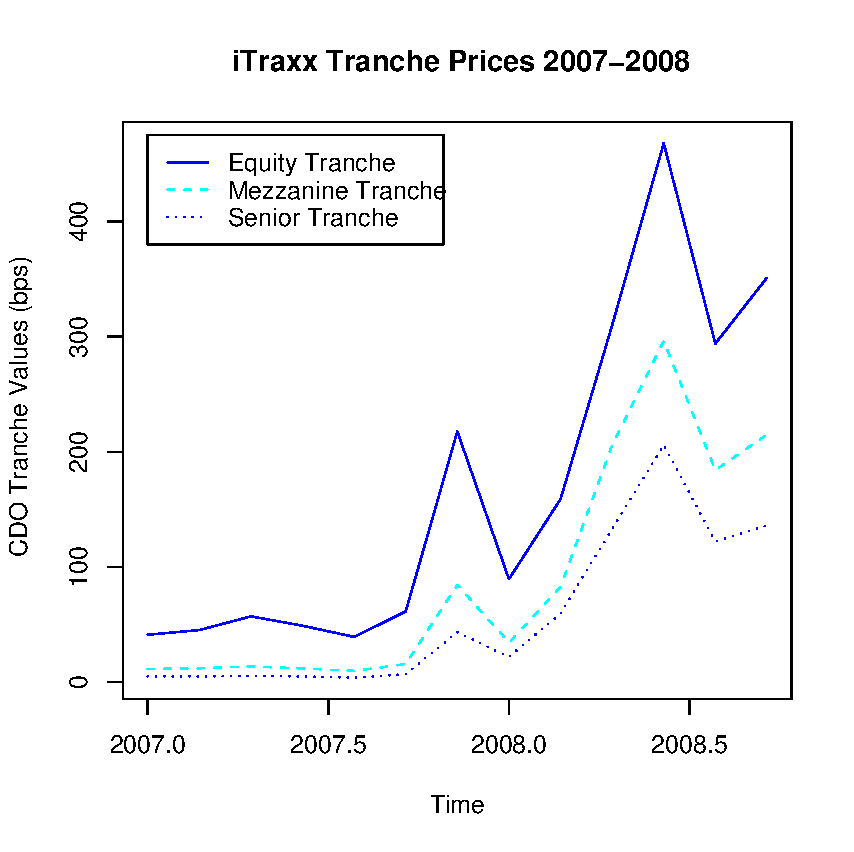
\includegraphics{pictures/iTraxxSpreads.pdf}}}
\caption{\label{table:trancheSpread}Changing Spreads on iTraxx.Europe index tranches from 01 Jan 2007 to 31 July 2008, source: \it{www.creditfixings.com}}
\end{figure}


As we can see from Figure~\ref{table:trancheSpread} the large jump in spreads occurred between June and July 2007 at the initiation of the credit crisis.  This followed reports on the 20th June that two Bear-Stearns managed hedge funds invested in securities backed by subprime mortgage loans were close to being shut down followed by, on the 10th July 2007, S \& P placing \$7.3 billion worth of 2006 vintage ABSs backed by residential mortgages on negative ratings watch and Moody's downgrading \$5bn worth of subprime mortgage bonds. Consequently, on the 11th July Moody's put 184 mortgage-backed on downgrade alert.

\cite{Green2005} presciently stated that "some observers ... are concerned that banks' efforts to lay off risk using credit derivatives may be creating concentrations of risk outside the banking system that could prove a threat to financial stability. A particular concern has been that, as credit spreads widen appreciably at some point from the extraordinarily low levels that have prevailed in recent years, losses to nonbank risk-takers could force them to liquidate their positions in credit markets and thereby magnify and accelerate the widening of credit spreads." It is standard practice for the originator of a CDO to retain the equity tranche. This is usually a bank intending to signal the riskiness of a deal whilst also serving to ensure prospective buyers that it will monitor credit payments.  \cite{Eli2006} notes that major banks do hold significant positions in the deals they construct and this is obviously a key factor in the losses suffered by these banks in the year 2007-2008.


\section{Outline \& Goals of this Report}\index{Outline}

In chapter~\ref{chap:review} we introduce and review Credit Derivatives, focussing on $N^{th}$-to-default Basket Swaps (NTDs) and Collateralised Debt Obligations (CDOs) and detail the prime risk-neutral mechanisms for pricing these products. Chapter~\ref{chap:study} details the practical investigation of this work whilst Chapter~\ref{chap:conclusion} concludes and attempts, and no more than that, to put into context the pricing issues with the market as seen over the period from June 2007 to August 2008.  Simulations for this report were implemented in the S programming language and executed on R 
(\url{http://www.r-project.org})
and S-plus (\url{http://www.insightful.com}) systems. Data was obtained from a number of sources, principally {\em Datastream} and \url{http://www.creditfixings.com}.
